%\documentclass{cmspaper}
%\begin{document}

\section{CMS Potential} \label{CMSpotential}

In order to estimate the potential of the CMS detector to discover the first generation leptoquarks
in the electron channel, a simple counting experiment approach is used. 
The number of signal and background events expected for an integrated luminosity of
$100\text{ pb}^{-1}$ listed in Table~\ref{tab:EventSelSummary} and the systematic uncertainties described 
in Section~\ref{sec:Systematics} are used to produce the following plots. 
The QCD background estimates from Table~\ref{tab:EventSelSummary} 
are not included due to lack of MC statistics. The QCD background is expected to be 
small compared to the other main background contributions (see Section~\ref{sec:QCDBackground}).

To quantify the significance of the
leptoquark signal, $S_\text{cP}$ significance estimator~\cite{ref:scp} is used. $S_\text{cP}$ assumes a Poisson distribution
with mean $b$ and gives the probability to observe $n=s+b$ events or greater
\begin{equation}
P = p(n\geq s+b|b) = \sum_{n=s+b}^{+\infty} \frac{b^n}{n!}e^{-b},
\end{equation}
where $s$ and $b$ are the expected numbers of signal and background events, respectively. This probability is 
converted into an equivalent number of standard deviations using the one-sided Gaussian probability
\begin{equation}
P = \frac{1}{\sqrt{2\pi}}\int_{S_\text{cP}}^{+\infty} e^{-\frac{x^2}{2}}\mathrm{d}x,
\label{eq:ScP}
\end{equation}
which gives the numerical value of the $S_\text{cP}$ significance. If the background has uncertainties, which we can express in terms of
a probability density function $f(b)$, the probability to observe $n=s+b$ events or greater becomes
\begin{equation}
P = \int_0^{+\infty} p(n\geq s+b|b)f(b)\mathrm{d}x,
\end{equation}
and the final $S_\text{cP}$ significance is again obtained using Eq.~\ref{eq:ScP}. Figure~\ref{fig:discovery} shows the required integrated luminosity
for a $5\sigma$ discovery for different leptoquark mass hypotheses. Figure~\ref{fig:discovery_beta} shows the minimum $\beta^2$ for
a $5\sigma$ discovery as a function of leptoquark mass for $100\text{ pb}^{-1}$ of integrated luminosity.

\begin{figure}[h!]
 \centering
  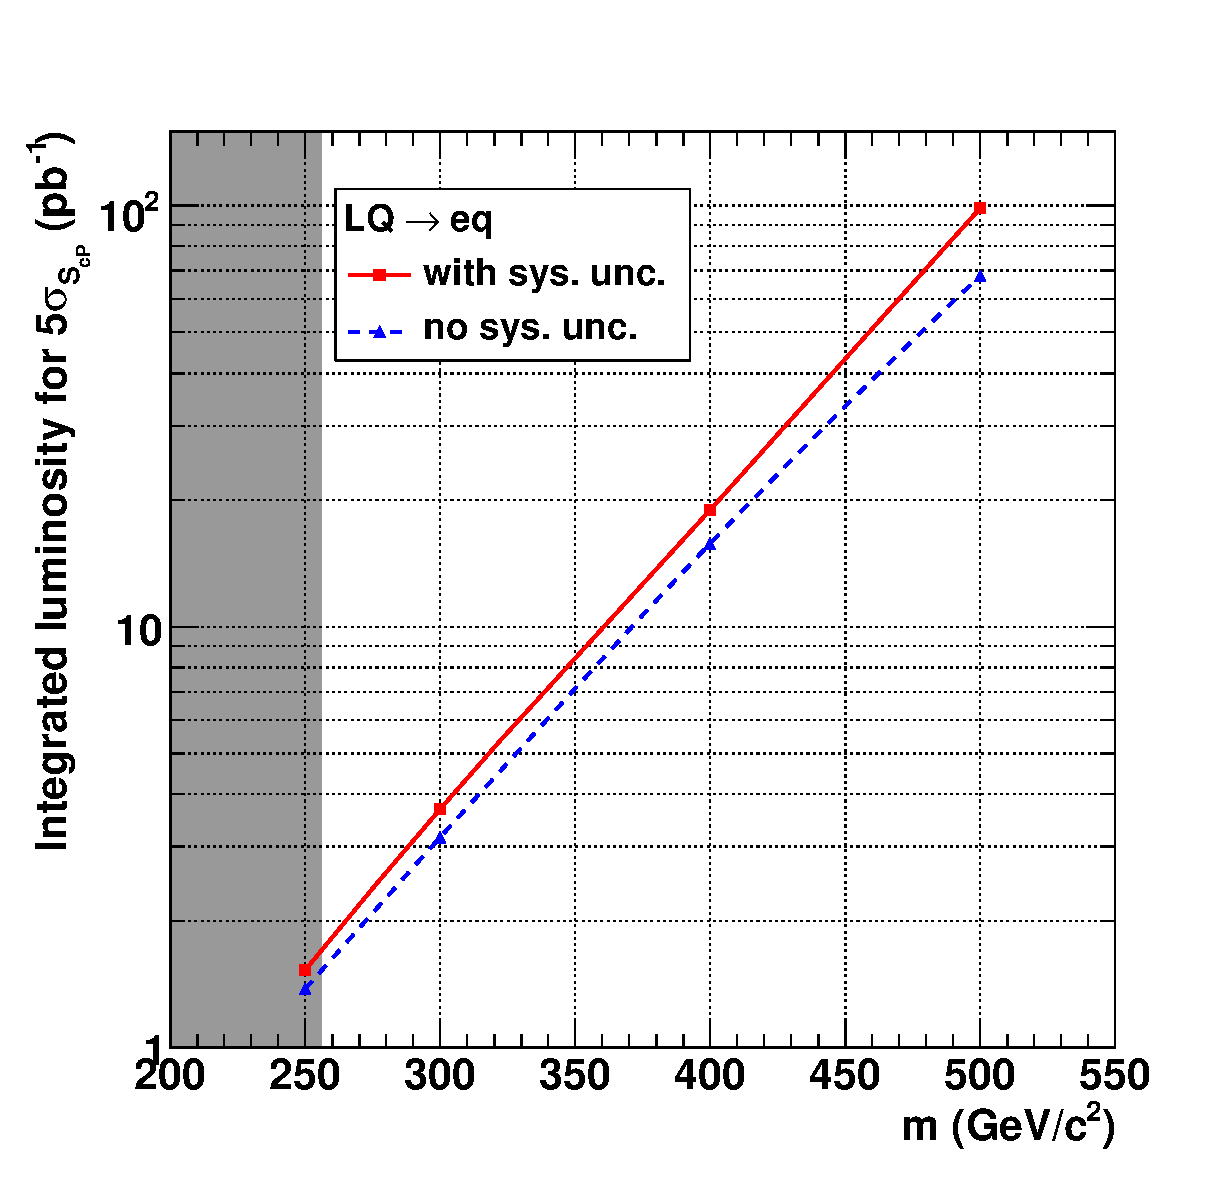
\includegraphics[width=0.5\textwidth]{plots/cmsPotential/L5sigma_vs_m_log.eps}
 \caption{\small \sl Integrated luminosity
for a $5\sigma$ discovery for different leptoquark mass hypotheses assuming $\beta=1$. Solid red line includes the systematic uncertainties described in 
Section~\ref{sec:Systematics}. Shaded region is excluded by the current Tevatron limits.\label{fig:discovery}}
\end{figure}
\begin{figure}[h!]
 \centering
  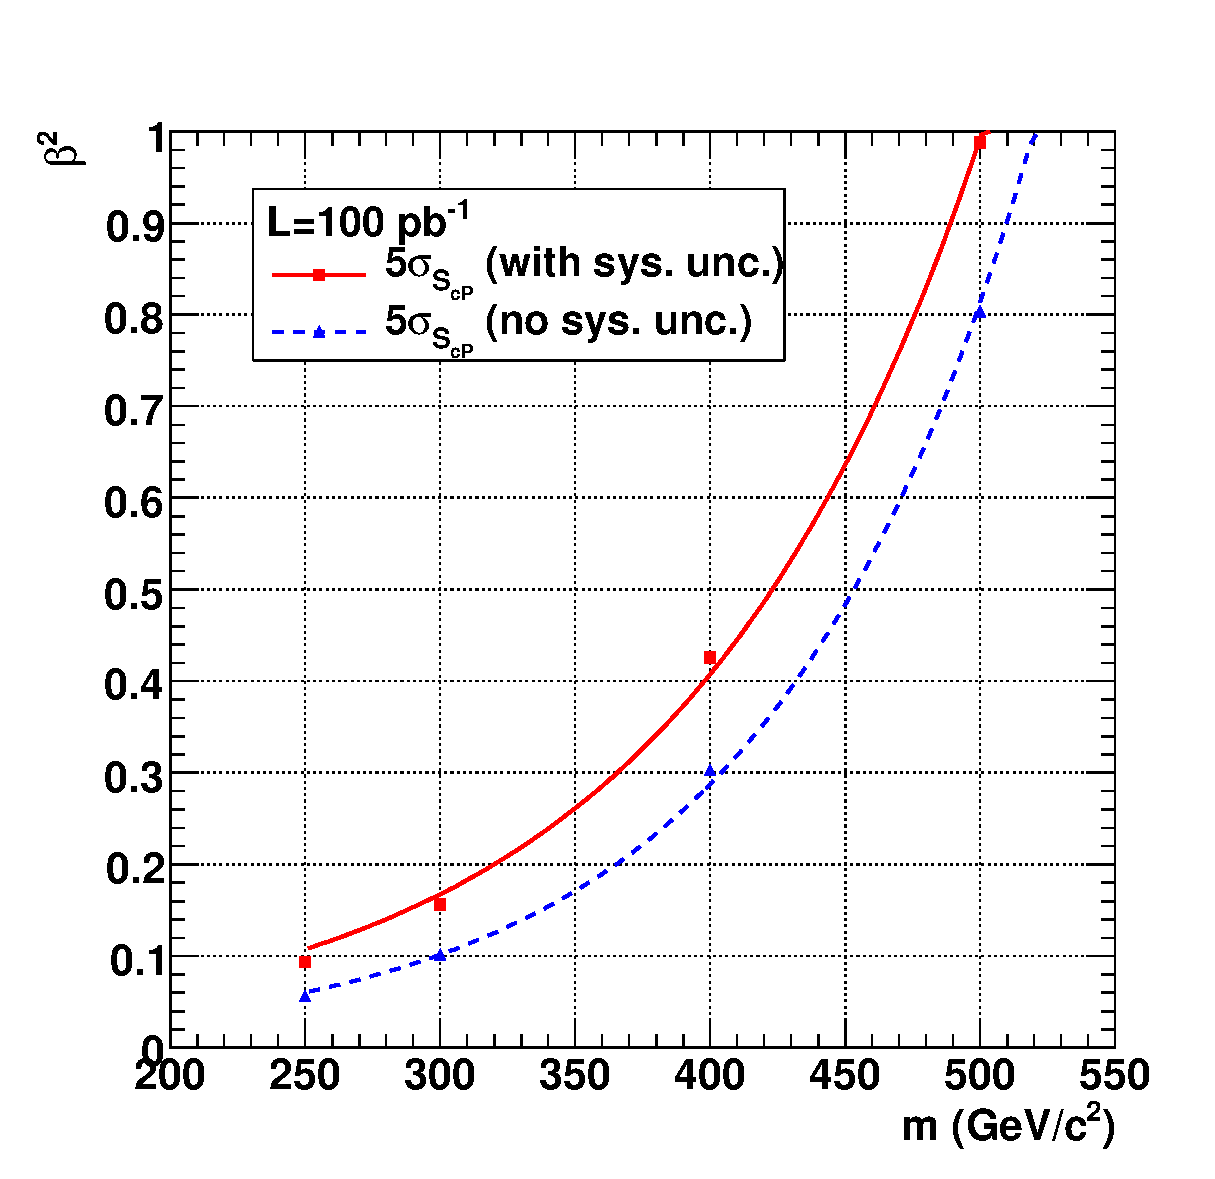
\includegraphics[width=0.5\textwidth]{plots/cmsPotential/beta2_vs_m.eps}
 \caption{\small \sl Minimum $\beta^2$ for
a $5\sigma$ discovery as a function of leptoquark mass for $100\text{ pb}^{-1}$ of integrated luminosity. Solid red line includes the systematic
uncertainties described in Section~\ref{sec:Systematics}.\label{fig:discovery_beta}}
\end{figure}


For setting upper limits in the absence of the leptoquark signal, the Bayesian approach~\cite{ref:bayes} is used. In this approach, the
posterior probability density function for the signal mean $s$, given $n$ observed events,
\begin{equation}
p(s|n)=\frac{L(n|s)\pi(s)}{\int_0^{+\infty}L(n|s)\pi(s)\mathrm{d}s},
\end{equation}
where $L(n|s)$ is a Poisson distribution
\begin{equation}
L(n|s)=\frac{(s+b)^n}{n!}e^{-(s+b)},
\end{equation}
and $\pi(s)$ is the prior for the signal mean $s$, is used to set up an upper limit on the leptoquark pair production cross section.
An upper limit $s_\text{up}$ at $95\%$ C.L. is obtained by requiring
\begin{equation}
\int_{-\infty}^{s_\text{up}}p(s|n)\mathrm{d}s=\frac{\int_{-\infty}^{s_\text{up}}L(n|s)\pi(s)\mathrm{d}s}{\int_{-\infty}^{+\infty}L(n|s)\pi(s)\mathrm{d}s}=0.95, 
\end{equation}
where one often uses
\begin{equation}
\pi(s)=\begin{cases}
          0&  s<0,\\
          1&  s\geq 0,
\end{cases}
\end{equation}
which effectively sets the lower limit of integration to zero. Since there is no actual observation, the expected 
upper limit $\mathrm{<}s_\text{up}\mathrm{>}$ in the background-only hypothesis is calculated as follows
\begin{equation}
\mathrm{<}s_\text{up}\mathrm{>}=\sum_{n=0}^{+\infty} s_\text{up}(n)L(n|s=0).
\end{equation}
This approach also allows for inclusion of systematic uncertainties which are treated as \emph{nuisance parameters} $\bm{\nu}$.
A modified posterior probability density function obtained by integrating over the nuisance parameters
\begin{equation}
L'(n|s)=\int L(n|s)\pi(\bm{\nu})\mathrm{d}\bm{\nu}
\end{equation}
is used instead of $L(n|s)$ to incorporate systematic uncertainties into the final result for an upper limit. Figure~\ref{fig:exclusion}
shows the required integrated luminosity for $95\%$ C.L. exclusion of different leptoquark mass hypotheses. Figure~\ref{fig:exclusion_xs}
shows the expected $95\%$ C.L. upper limit on the leptoquark pair production cross section as a function of leptoquark mass for $100\text{ pb}^{-1}$
of integrated luminosity. 
%The number of signal and background events expected for an integrated luminosity of
%$100\text{ pb}^{-1}$ listed in Table~\ref{tab:EventSelSummary} and the systematic 
%uncertainties described in Section~\ref{sec:Systematics} are used to produce the plots.

\begin{figure}[h!]
 \centering
  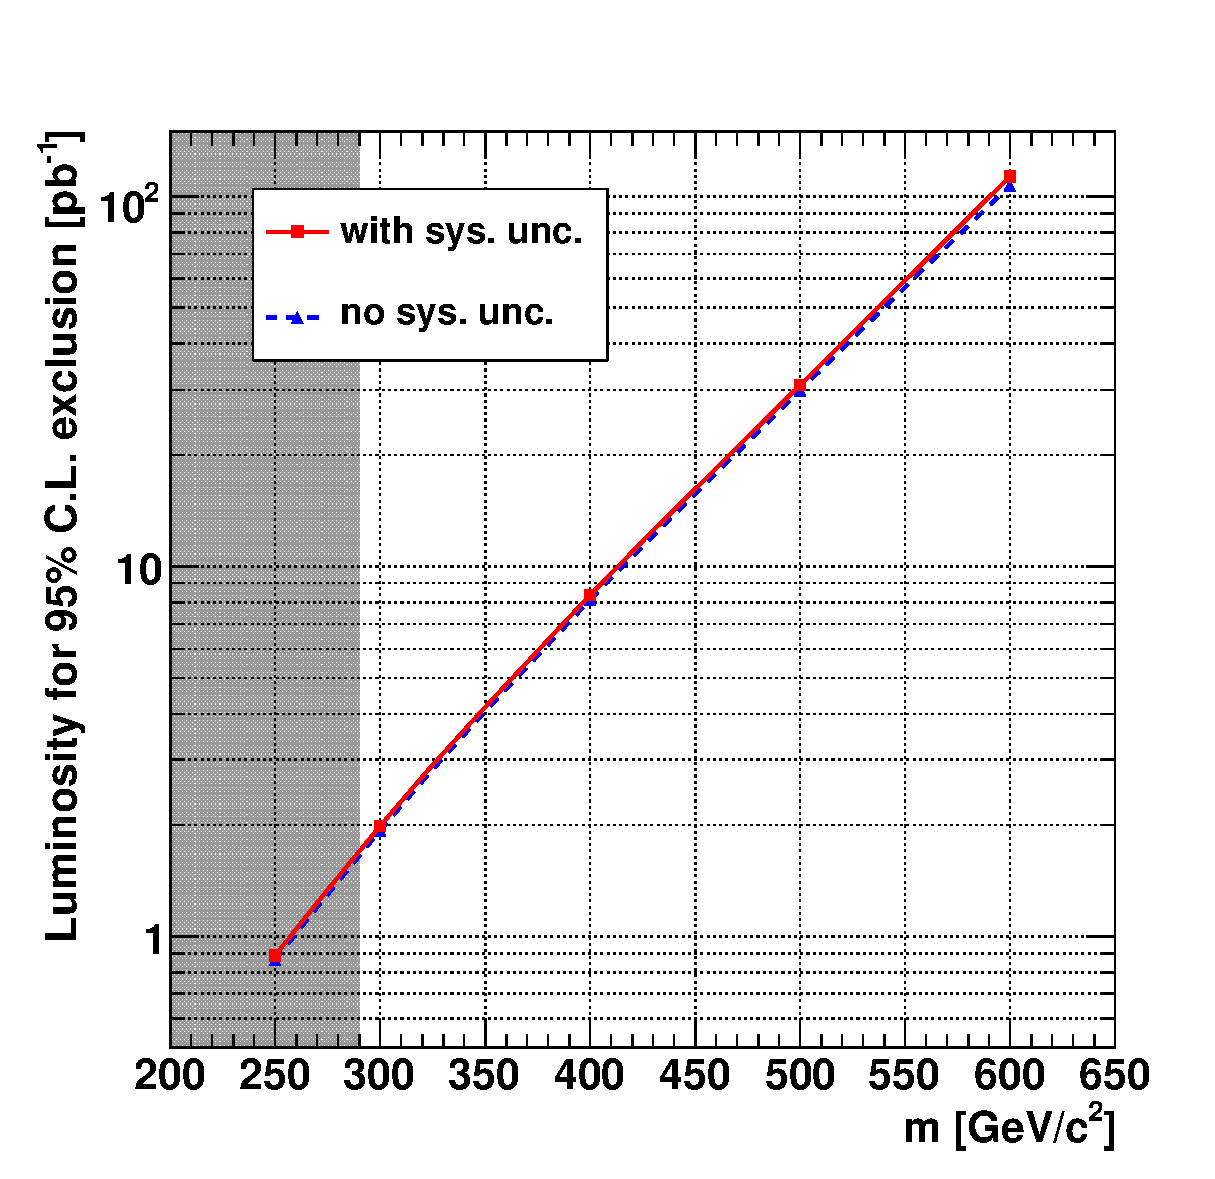
\includegraphics[width=0.5\textwidth]{plots/cmsPotential/L95CL_vs_m_log.eps}
 \caption{\small \sl Integrated luminosity
for $95\%$ C.L. exclusion of different leptoquark mass hypotheses assuming $\beta=1$. Solid red line includes the systematic
uncertainties described in Section~\ref{sec:Systematics}. Shaded region is excluded by the current Tevatron limits.\label{fig:exclusion}}
\end{figure}
\begin{figure}[h!]
 \centering
  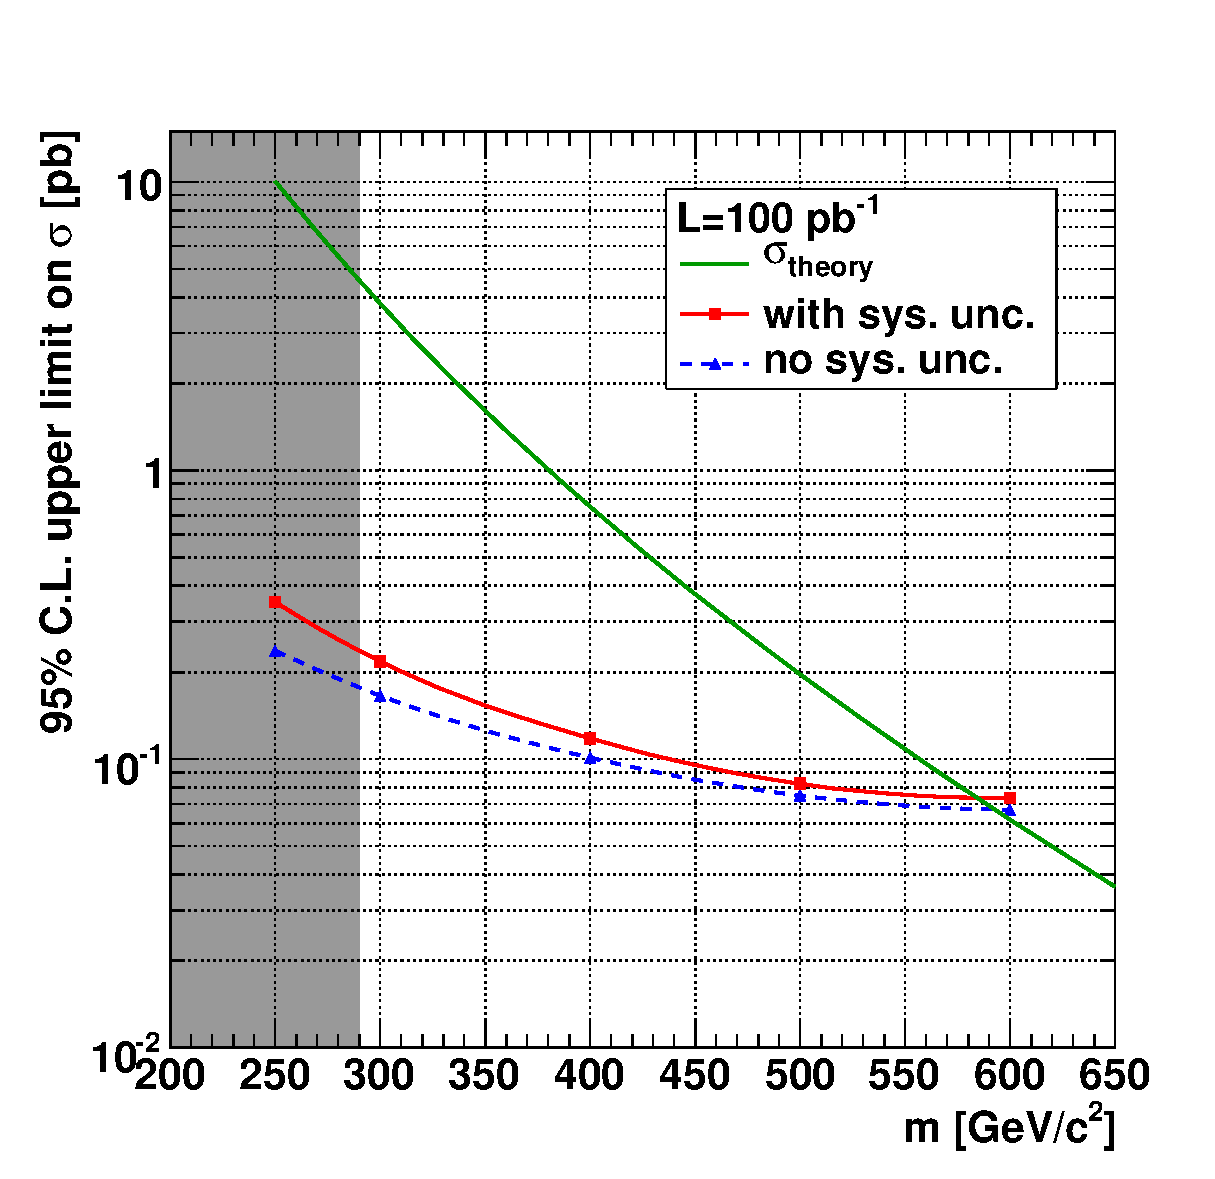
\includegraphics[width=0.5\textwidth]{plots/cmsPotential/xs95CL_vs_m_log.eps}
 \caption{\small \sl Expected $95\%$ C.L. upper limit on the leptoquark pair production cross section as a function of leptoquark mass for $100\text{ pb}^{-1}$
of integrated luminosity assuming $\beta=1$. Solid red line includes the systematic uncertainties described in Section~\ref{sec:Systematics}.
Shaded region is excluded by the current Tevatron limits.
\label{fig:exclusion_xs}}
\end{figure}


%\subsection{Discovery Luminosity}

% In order to estimate the integrated luminosity needed by CMS to claim 
% a discovery in the electron channel of the first generation leptoquark
% several MC experiments with signal and background events are produced
% as described in section \ref{sec:signalExtraction}.
% 
% The significance of each experiment is extracted using the log-likelihood estimator 
% \begin{displaymath}
% S_L \equiv \sqrt{2\cdot ln{(L_{s+b}/L_{b})}}~\mathrm{,}
% \end{displaymath}
% where $L_{s+b}$ and $L_b$ are the maximum likelihood values for the fit to
% the signal plus background and background only hypothesis, respectively.
% 
% A set of MC experiments is generated for a leptoquark mass and a value of 
% the integrated luminosity.
% The distribution of $S_L$ of the set of experiments is approximately gaussian 
% and its median is used as the estimate of the significance.
% The procedure is repeated for leptoquark masses of 250, 400 and 650~GeV and
% different values of the integrated luminosity. The results are shown in
% Figure~\ref{fig:sign_vs_Lint_sysR}, which includes also the effect of the systematic 
% uncertainties discussed in the next section. 

% \begin{figure}
%   \begin{center}
%     \resizebox{7cm}{!}{\includegraphics{plots/significanceDistribution.eps}}
%     \caption{\small \sl significanceDistribution}
%     \label{fig:significanceDistribution}
%   \end{center}
% \end{figure}

% \begin{figure}
%   \begin{center}
%     \resizebox{10cm}{!}{\includegraphics{plots/significanceVsIntLum.eps}}
%     \caption{\small \sl Significance of the discovery as a function of integrated luminosity.
%     The curves represents fits to the points of a certain leptoquark mass using a 
%     square root function. The horizontal line represents a 5 sigma discovery.}
%     \label{fig:significanceVsIntLum}
%   \end{center}
% \end{figure}

% \subsection{Systematic uncertainties}

%The impact of systematic effects on the discovery potential and the determination 
%of the experiment sensitivity are not yet included in this study.

%A study for determining the sensitivity of the experiment will be performed.
%It will be used to set upper limits in case a signal is not observed. 
%It will be used an approach similar to the one used in \ref{highmassToMuons}.
%The same tools to generate MC experiments and perform log-likelihood fits will be used.

%Systematics: Luminosity(+_10\%), JES (+_10\%), ratio ttbar/Zgammajets, etc.

% The method used to discriminate between signal and background events and extract the significance 
% of a possible observed leptoquark signal 
% relies on the knowledge of the shape of the signal and background distributions 
% by fitting the $M_{ej}$ distribution of the eejj sample.
% The shape of the background distributions will be determined from the data as 
% described in section~\ref{sec:bkgStudy}.
% As a consequence, once real data is available, the uncertainty on the knowledge of quantities 
% such as the integrated luminosity, the efficiency of the signal selection, the signal cross section, 
% and the magnitude of the total background cross section, will not have an impact on the 
% determination of the significance.
% On the other hand, uncertainties that affect the knowledge of the shape of the distributions of 
% the total background and the signal will have an impact on the significance and have to be 
% accounted for as systematic uncertainties.
% 
% The value of $R$, defined in section \ref{sec:signalExtraction} as 
% the ratio between the number of $t\bar{t}$ and $Z/\gamma$+jets events in the final sample,
% directly affects the shape of the total background distribution used in the fit by changing the
% mixture of the two backgrounds. 
% Hence, the impact of the uncertainty on its value has to be included in the significance systematics.
% The current knowledge, $R_{MC}$, of $R$ comes from the Monte Carlo
% study and may introduce a deviation $\delta \equiv R/R_{MC}$ from the true value of $R$
% due, for example, to imperfect knowledge of the relative magnitude of the two background 
% cross sections and respective selection efficiencies.
% 
% Once real data is available there will be a way to infer the departure of $\delta$ from unity.
% If $\tilde{R}$ is defined as the ratio between the number of $t\bar{t}$ and $Z/\gamma$+jets events in the
% control samples described in section~\ref{sec:bkgStudy} and $\tilde{R}_{MC}$ is its
% estimate from Monte Carlo, it is reasonable to expect that the main reasons that
% make $\delta$ deviate from unity do affect $\tilde{R}/\tilde{R}_{MC}$ in the same way.
% This is because the largest uncertainties of the MC are expected to come from the estimate 
% of the cross section of the $t\bar{t}$ and $Z/\gamma$+jets processes, 
% which affects equally $\tilde{R}_{MC}$ and $R_{MC}$.
% Therefore, it can be concluded that $\delta \simeq \tilde{R}/\tilde{R}_{MC}$ and, once real data is available
% to calculate $\tilde{R}$ from the control samples of $t\bar{t}$ and $Z/\gamma$+jets, this estimate 
% of $\delta$ will be used to improve the knowledge of $R$ from the current estimate, $R_{MC}$, 
% to $R_{data+MC} \equiv \delta \cdot R_{MC}$.
% The significance fit will then be done using $R_{data+MC}$. 
% 
% The uncertainty on the estimate of $\delta$ given by $\tilde{R}/\tilde{R}_{MC}$ will be 
% dominated by the statistical error of $\tilde{R}$ from the number of events in the control samples. 
% This will propagate to give an uncertainty $\Delta R_{data+MC}$ on $R_{data+MC}$ and will
% be larger for small integrated luminosities. 
% Currently, $\Delta R_{data+MC}$ is estimated using the CSA07 control samples.
% The fit to extract the significance is here repeated changing the value of $R$ by 
% $\pm\Delta R_{data+MC}$ from its central value $R_{MC}$ \footnote{Not having real data yet, 
% exact correctness of the MC is currently assumed by setting $\delta=1$, 
% making effectively $R_{data+MC}=R_{MC}$.}, and the results are shown in 
% Figure~\ref{fig:sign_vs_Lint_sysR}.
% The systematic uncertainty due to $R$ is larger, for the same integrated luminosity, for a
% LQ mass of 250~GeV. This is due to the topology of the $M_{ej}$ distribution 
% of the signal that, at small LQ masses, peaks where the background does.
% For higher values of the LQ mass, the significance determination seems to be little 
% sensible to variations of $R$. This may be understood by considering the increased separation
% between the main features of the signal and background distributions, and the relative similarity 
% between the two background shapes: 
% the mixture between $t\bar{t}$ and $Z/\gamma$+jets events may vary, but
% the mixture between total background and signal does little.
% As an example, for the point at $M_{LQ}=400$~GeV, integrated luminosity=100~$pb^{-1}$ and significance=12.7
% the uncertainty  $\Delta R_{data+MC}$ is about 15\%, but this determines a change of 
% significance of only 1\%.
% 
% The fact that, apart from the small LQ mass region and low luminosity scenario where special care
% will have to be applied, the uncertainty 
% of $R$ tends to be ``absorbed'' in the fitting procedure and have a limited impact on the 
% significance determination indicates that this systematics is reasonably under control. 
% In addition, it reassures that once the real data is available and the value of the correction 
% factor $\delta$, currently set to unity, can be estimated as described above and used in the fit,
% even a significant departure from unity will not require a drastic re-assessment of
% the current estimate of the luminosity needed for discovery.
% The uncertainty on the knowledge of the signal shape used in the fit may also produce a systematic
% uncertainty on the significance. A study of this effect will have to be performed.
% 
%  \begin{figure}
%    \begin{center}
%      \resizebox{10cm}{!}{
\includegraphics{plots/UMD.eps}}
%      \caption{\small \sl Significance of the discovery as a function of the integrated luminosity.
%        For each LQ mass, the fit to extract the significance is repeated varying the value of $R$
%        (the ratio between the number of $t\bar{t}$ and $Z/\gamma$+jets events in the final sample)
%        of an amount $\pm\Delta R_{data+MC}$ from its central value $R_{data+MC}$ 
%        (see text for details).
%        Apart from a couple of points at a LQ mass of 650~GeV, the higher curves correspond to
%        the higher value of $R$. 
%        The horizontal line represents a 5 sigma discovery.}
%      \label{fig:sign_vs_Lint_sysR}
%    \end{center}
%  \end{figure}
% 
% In the case of setting an upper limit in the case of absence of signal, a larger number of systematic
% uncertainties will have to be considered as they do have a direct impact on it. 
% Such uncertainties include the one on the integrated luminosity, the detector efficiency and 
% resolution, the jet energy scale, and theoretical uncertainties such as those on parton distributions
% and higher-order corrections on the cross sections. Different scenarios of levels of background
% and signal will have to be studied. The procedure for setting an upper limit and the study of the 
% systematics involved is not yet included in this version of the analysis.



%\end{document}
